\documentclass[12pt,a4paper]{article}
%\documentclass[11pt,UTF8]{article}
%\usepackage{ctex}
\usepackage{tcolorbox}
\usepackage{graphicx}
\usepackage{geometry}
\usepackage{listings}
\usepackage{xcolor}
\usepackage{mathtools}
\usepackage{framed} 
\usepackage{amsfonts}
\usepackage{algpseudocode} 
\usepackage{algorithm}
\usepackage{ulem}
\usepackage{tikz}

\renewcommand{\algorithmicrequire}{ \textbf{Input:}} %Use https://www.overleaf.com/project/6038f72fd2827e6248936428Input in the format of Algorithm
\renewcommand{\algorithmicensure}{ \textbf{Output:}} %Use Output in the format of Algorithm
\definecolor{codegreen}{rgb}{0,0.6,0}
\definecolor{codegray}{rgb}{0.5,0.5,0.5}
\definecolor{codepurple}{rgb}{0.58,0,0.82}
\definecolor{backcolour}{rgb}{0.95,0.95,0.92}

\usepackage{tikz}
\usepackage{tikz-qtree}

\begin{document}
\noindent

%========================================================================
\noindent\framebox[\linewidth]{\shortstack[c]{
\Large{\textbf{Homework 4}}\vspace{1mm}\\
VE216 - Introduction to Signal and Systems, Qiao Heng, Spring 2021}}

\begin{center}

\footnotesize{\color{blue}$*$ Name: Han Yibei \quad\quad\quad\quad\quad Student ID: 519370910123}
\end{center}

\section*{HW Notes:}
\begin{itemize}
    \item Problems where the number of points are followed by an exclamation are basic skill problems and will be graded without partial credit.
    \item \fbox{Box} your final answer. You will be graded on both the final answer and the steps leading to it. Correct intermediate steps will help earn partial credit.
    For full credit, \sout{cross out} any incorrect intermediate step.
    \item If you need to make any additional assumptions, state them clearly.
    \item Legible writing will help when it comes to partial credit.
    \item Simplify your result when possible.
\end{itemize}

\section*{Problems:}
\normalsize
\begin{tcolorbox}[colback = white]
1. [20!] Use the table of FT pairs and the table of properties to find the FT of each of the following signals (DO NOT USE INTEGRATION):\\
(a) $[5 !] x(t)={rect}\left(\frac{t-1}{2}\right)$\\
(b) $[5 !] x(t)=e^{-3 t} {rect}\left(\frac{t-1}{2}\right)$\\
(c) $[5 !] x(t)={trect}\left(\frac{t-1}{2}\right)$\\
(d) $[5 !] x(t)=\cos (2 \pi t) {rect}\left(\frac{t-1}{2}\right)$

\end{tcolorbox}

\begin{tcolorbox}
\normalsize
\textcolor{blue}{Answer:\\
(a)$f(t)={rect}\left(\frac{t}{T}\right)\text{so }F(\omega)=T {sinc}\left(T \frac{\omega}{2 \pi}\right) \text { , }$\\
    $\text { suppose } h(t)={rect}\left(\frac{t}{2}\right) \quad H(\omega)=2 {sinc}\left(\frac{\omega}{\pi}\right)$\\
    $x(t)=h(t-1), X(\omega)=H(\omega) e^{-j \omega}=\fbox{$2 e^{-j \omega} {sinc}\left(\frac{\omega}{\pi}\right)$}$\\
(b) $x(t)=e^{-3t}u(t)-e^{-3t}u(t-2)$\\
$X(\omega)=\fbox{$\frac{1}{j\omega+3}+\frac{e^{-6-j\omega2}}{j\omega+3}$}$\\
(c) $ h(t)={rect}\left(\frac{t-1}{2}\right)~~~H(\omega)=2 e^{-j \omega} 4{sinc}\left(\frac{\omega}{\pi}\right)$\\
$x(t)=th(t)=j(-jt)h(t)=j\frac{d}{d\omega}~~~~F(\omega)=\fbox{$\frac{(1+2 j \omega) e^{-2 j \omega}-1}{\omega^{2}}$}$\\
(d) $X(\omega)=\frac{H(\omega-2\pi)+H(\omega+2\pi)}{2}=\fbox{$e^{-j \omega} \sin \omega \frac{2 \omega}{\omega^{2}-4 \pi^{2}}$}$
}
\end{tcolorbox}

\begin{tcolorbox}[colback = white]
2. [10] Find a mathematical expression and sketch or plot the inverse $\mathrm{FT}$ of $F(\omega)={sinc}^{3}(\omega / 2)$. Hint: the inverse FT formula would probably be a hard way to do it.
\end{tcolorbox}

\begin{tcolorbox}
\normalsize
\textcolor{blue}{Answer:\\
when $h(t)=\frac{1}{\pi}rect(\frac{t}{\pi})$, $H(\omega)=sinc(\frac{\omega}{2})$\\
So if $F(\omega)=H(\omega)^3$, then $f(t)=h(t)*h(t)*h(t)=\frac{1}{\pi^2}tri(\frac{t}{\pi})*rect\frac{t}{\pi}$\\
$$
\fbox{f(t)}=\left\{\begin{array}{ccc}
0 & t \leq-\frac{3}{2} \pi \\
\frac{1}{2 \pi^{3}} t^{2}+\frac{3}{2 \pi^{2}} t+\frac{9}{8 \pi}  & -\frac{3}{2} \pi \leq t \leq-\frac{\pi}{2}\\
\frac{3}{4 \pi}-\frac{t^{2}}{\pi^{3}} & -\frac{\pi}{2} \leq t \leq \frac{\pi}{2} \\
\frac{1}{2 \pi^{3}} t^{2}-\frac{3}{2 \pi^{2}} t+\frac{9}{8 \pi} & \frac{\pi}{2} \leq t \leq \frac{3 \pi}{2} \\
0 & t \geq \frac{3}{2} \pi
\end{array}\right.
$$
\begin{figure}[H]
    \centering
    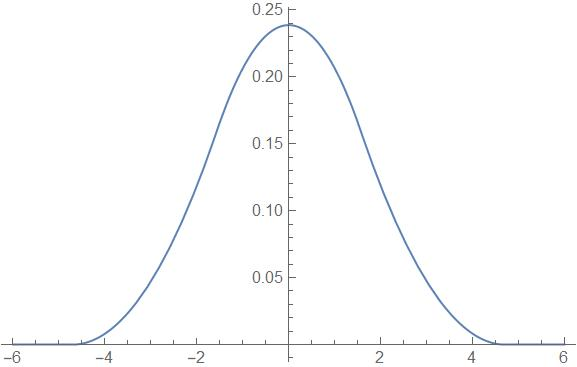
\includegraphics[width=8cm]{2.jpg}
\end{figure}
}
\end{tcolorbox}

\begin{tcolorbox}[colback = white]
3. [10] Find the FT of $t^{2} e^{-(t / 4)^{2}}$. Hint: see table of FT pairs.
\end{tcolorbox}

\begin{tcolorbox}
\normalsize
\textcolor{blue}{Answer:\\
$x(t)=-(-jt)^2e^(-\frac{t}{4})^2$\\
so $X(\omega)=-\frac{d^2}{d\omega^2}(4\sqrt{\pi}e^{-4\omega^2})=\fbox{$32\sqrt{\pi}e^{-4\omega^2}(1-8\omega^2)$}$
}
\end{tcolorbox}

\begin{tcolorbox}[colback = white]
4. [10] Show that if $f(t)$ is real and odd, then $F(\omega)$ is purely imaginary and odd.
\end{tcolorbox}

\begin{tcolorbox}
\normalsize
\textcolor{blue}{Answer:\\
f(t) is odd, so $f(t)+f(-t)=0$, then $f(t)+f(-t) \stackrel{\mathcal{F}}{\longleftrightarrow} F(\omega)+F(-\omega)=0$, so $F(\omega)$ is odd\\
f(t) is real, so $f(t)-f*(t)=0$, then $f(t)-f*(t) \stackrel{\mathcal{F}}{\longleftrightarrow} F(\omega)-F*(\omega)=0$, so $F(\omega)$ is real
}
\end{tcolorbox}


\begin{tcolorbox}[colback = white]
5. [10] Consider a real signal $f(t)$ and let
$$
f(t) \stackrel{\mathcal{F}}{\leftrightarrow} F(\omega), \quad F(\omega)={real}\{F(\omega)\}+j {imag}\{F(\omega)\}
$$
and
$$
f(t)=f_{e}(t)+f_{o}(t)
$$
where $f_{e}(t)$ and $f_{o}(t)$ are the even and odd component of $f(t)$ respectively. Show that
$$
f_{e}(t) \stackrel{\mathcal{F}}{\leftrightarrow} {real}\{F(\omega)\} \quad f_{o}(t) \stackrel{\mathcal{F}}{\longleftrightarrow} j {imag}\{F(\omega)\}
$$
\end{tcolorbox}

\begin{tcolorbox}
\normalsize
\textcolor{blue}{Answer:\\
$f(t)\stackrel{\mathcal{F}}{\longleftrightarrow} F(\omega)$, so $f_e(t)+f_o(t)\stackrel{\mathcal{F}}{\longleftrightarrow} F_e(\omega)+F_o(\omega)$\\
As in problem 4, $f_o(t)$ is odd and real, so $F_o(\omega)$ is odd and real\\
Also, f(t) is even, so $f(t)-f(-t)=0$, then $f(t)-f(-t) \stackrel{\mathcal{F}}{\longleftrightarrow} F(\omega)-F(-\omega)=0$, so $F(\omega)$ is even\\
f(t) is real, so $f(t)-f*(t)=0$, then $f(t)-f*(t) \stackrel{\mathcal{F}}{\longleftrightarrow} F(\omega)-F*(\omega)=0$, so $F(\omega)$ is real\\
So $f_e(t)$ is even and real, so $F_e(\omega)$ is even and real\\
So, $f_{e}(t) \stackrel{\mathcal{F}}{\leftrightarrow} {real}\{F(\omega)\} \quad f_{o}(t) \stackrel{\mathcal{F}}{\longleftrightarrow} j {imag}\{F(\omega)\}$
}
\end{tcolorbox}


\begin{tcolorbox}[colback = white]
6. [10!] Find the energy of the signal $x(t)=t {sinc}^{2}(t)$ by Fourier methods.
\end{tcolorbox}

\begin{tcolorbox}
\normalsize
\textcolor{blue}{Answer:\\
$sinc^2(t)\stackrel{\mathcal{F}}{\longleftrightarrow}tri(\frac{\omega}{2\pi})$\\
$$
\begin{aligned}
t \sin c^{2}(t) \stackrel{\mathcal{F}}{\longleftrightarrow} & j \frac{d}{d \omega} {tri}\left(\frac{\omega}{2 \pi}\right) \\
&=\frac{j}{2 \pi} \frac{d}{d \omega} {rect}\left(\frac{\omega}{2 \pi}\right) * {rect}\left(\frac{\omega}{2 \pi}\right) \\
&=\frac{j}{2 \pi}(\delta(\omega+\pi)-\delta(\omega-\pi)) * {rect}\left(\frac{\omega}{2 \pi}\right) \\
&=\frac{j}{2 \pi}\left({rect}\left(\frac{\omega+\pi}{2 \pi}\right)-{rect}\left(\frac{\omega-\pi}{2 \pi}\right)\right) \\
|X(\omega)| &=\frac{1}{2 \pi} {rect}\left(\frac{\omega}{4 \pi}\right)
\end{aligned}
$$
$E=\frac{1}{2\pi}\int_{-\infty}^\infty|X(\omega)|^2d\omega=\fbox{$\frac{1}{2\pi^2}$}$
}
\end{tcolorbox}

\begin{tcolorbox}[colback = white]
7. [10] What percentage of the total energy in the energy signal $f(t)=e^{-t} u(t)$ is contained in the frequency band $-8 \mathrm{rad} / \mathrm{s} \leq \omega \leq 8 \mathrm{rad} / \mathrm{s}$
\end{tcolorbox}
\begin{tcolorbox}
\normalsize
\textcolor{blue}{Answer:\\
$X(\omega)=\frac{1}{j\omega-1}$, so $E_{part}=\frac{1}{2\pi}\int_{-8}^8|F(\omega)|^2d\omega=\frac{arctan(8)}{\pi}$\\
$$E=\frac{1}{2\pi}\int_{-\infty}^\infty|F(\omega)|^2d\omega=\frac{1}{2}$$
$$P=\frac{E_{part}}{E}=\fbox{92\%}$$
}
\end{tcolorbox}


\begin{tcolorbox}[colback = white]
8. [20] A LTI system has the following frequency response:
$$
H(j \omega)=\frac{-\omega^{2}+j \omega+1}{\left(-\omega^{2}+6 j \omega+25\right)(j \omega+2)}
$$
(a) [10] Find the impulse response of the LTI system. Hint: first find the partial differential equation.\\
(b) [10] Find the differential equation corresponding to the LTI system. Hint: write $H(\omega)=Y(\omega) / X(\omega)$ and cross multiply.
\end{tcolorbox}
\begin{tcolorbox}
\normalsize
\textcolor{blue}{Answer:\\
(a) $H(s)=\frac{s^2+s+1}{(s^2+6s+25)(s+2)}$\\
$\frac{b}{s+3-4 j}+\frac{c}{s+3+4 j}+\frac{a}{s+2}=\frac{s^{2}+s+1}{\left(s^{2}+6 s+25\right)(s+2)}$
$
\Rightarrow
a=\frac{3}{17}~~
b=\frac{7}{17}+\frac{71}{136} j~~
c=\frac{7}{17}-\frac{71}{136} j
$\\
h(t)=\fbox{$\left(\frac{7}{17}+\frac{71}{136} j\right) e^{(4 j-3) t} u(t)+\left(\frac{7}{17}-\frac{71}{136} j\right) e^{(-4 j-3) t} u(t)+\frac{3}{17} e^{-2 t} u(t)$}\\
(b)
$$
\frac{Y(\omega)}{X(\omega)}=\frac{-\omega^{2}+j \omega+1}{\left(-\omega^{2}+6 j \omega+25\right)(j \omega+2)}$$
$$
\left(s^{3}+8 s^{2}+37 s+50\right) Y(\omega)=\left(s^{2}+s+1\right) X(\omega)
$$
$$\fbox{$y^{\prime \prime \prime}(t)+8 y^{\prime \prime}(t)+37 y^{\prime}(t)+50 y(t)=x^{\prime \prime}(t)+x^{\prime}(t)+x(t)$} 
$$
}

\end{tcolorbox}

%========================================================================
\end{document}
